\section{Introduction}
A powerful approach to process large heterogeneous sources of data is to use graph encodings [1], [8] and then use graph-based learning systems. In these systems the notion of node similarity is key. A common approach is to resort to graph node kernels such as diffusion-based kernels [2] where the graph node kernel measures the proximity between any pair of nodes by taking into account the paths that connect them. However, when the graph structure is affected by
noise in the form of missing links, node similarities are distorted proportionally to the sparsity of the graph and to the fraction of missing links. Two of the main reasons for this are that 1) the lower the average node degree is, the smaller the number of paths through which information can travel, and 2) missing links can end up separating a graph into multiple disconnected components. In this case, since information cannot travel across disconnected components, the similarity of nodes belonging to different components is null. To address these problems we propose to solve a link prediction task prior to the node similarity computation and start studying the question: how can we improve node similarity using link prediction? In this work we review both the link prediction literature and the diffusion kernel literature, select a subset of approaches in both categories that seem well suited, focus on a set of node predicting problems in the bioinformatics domain and empirically investigate the effectiveness of the combination of these approaches on the given predictive tasks. 

\section{Related work}
\section{Methods}
\subsection{Definitions and notation}
We represent a problem instance as a graph $G=(V,E)$ where $V$ is the set of nodes and $E$ is the set of links. The set $E$ is partitioned into the subset of observed links ($O$) and the subset of unobserved links ($U$). Like other approaches we assume that all unobserved links are indeed ``non-links'' and we therefore define the link prediction problem as the task of ranking candidate links from the most to the least probable to recover links in $O$ but not in $U$ exploiting only the network topology.


We define the \textit{distance} $\mathcal{D}(u,v)$ between two nodes $u$ and $v$, as the number of edges on the shortest path between them. The \textit{neighborhood} of a node $u$ with radius $r$, $N_r(u) = \lbrace v\ |\ \mathcal{D}(u,v) \leq r \rbrace$, is the set of nodes at distance no greater than $r$ from $u$. The corresponding \textit{neighborhood subgraph} $\mathcal{N}_{r}^{u}$ is the  subgraph induced by the neighborhood (i.e. considering all the edges with endpoints in $N_r(u)$). The \textit{degree} of a node $u$, $deg(u) = |\mathcal{N}_{1}^{u}|$, is the cardinality of its \textit{neighborhood}. The maximum node degree in the graph $G$ is $deg(G)$.
\subsection{Disjunctive interconnection graph integration}
\textit{Definitions.} A graph $G = (V,E)$ is a structure that consists of a node set $V(G)$ and an edge set $E(G)$. The \textit{distance} between two nodes $u$ and $v$, notated as $\mathcal{D}(u,v)$, is the length of the shortest path between them. The \textit{neighborhood} with radius $r$ of a node $v$ is the set of nodes
at a distance no greater than $r$ from $v$ and denoted by $N_r(v)$. The \textit{neighborhood subgraph} with radius $r$ of node $v$, denoted by $\mathcal{N}_{r}^{v}$,  is the subgraph formed by the nodes in the
neighborhood with radius $r$ of $v$ and the relative edges with endpoints in $N_r(v)$.

\subsubsection*{Network Decomposition} 
In gene-disease associations networks it is not uncommon to find nodes with high degrees. Unfortunately these cases cannot be effectively processed by decomposition kernels based on exact neighborhood matches
because of the high number of neighborhood subgraphs. As an alternative, we propose to decompose the network in a linked collection of sparse sub-networks where each node has a reduced connectivity. More precisely we distinguish two types of edges: {\em conjunctive} and {\em disjunctive} edges. Nodes linked by conjunctive edges are going to be used jointly to define the notion of context. Nodes linked by disjunctive edges are instead used to define features based only on the
pairwise co-occurrence of the genes at the endpoints. The aim of the following decompositions is to link sparse sub-networks (which comprise only conjunctive edges) via disjunctive edges. 

\textit{Iterative k-core decomposition} \cite{kcore}: The node set is partitioned in two groups on the basis of the degree of each node w.r.t. a threshold degree $D$. The node partition is used to induce the conjunctive vs disjunctive edge partition: edges that have endpoints in the same part are marked as conjunctive, while edges with endpoints in different parts are marked as disjunctive. We apply the k-core decomposition iteratively considering only the graph induced by the conjunctive edges until no node has a degree \footnote{The degree is defined by only considering incident conjunctive edges.}greater than $D$.

\begin{figure}
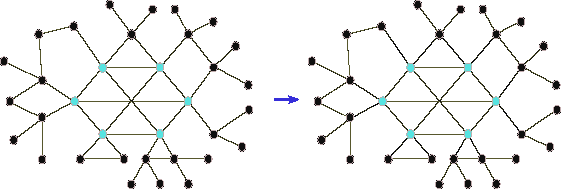
\includegraphics[height=1.1in, width=3in]{k_core.pdf}
\caption{K-core decomposition}
\label{fig:01}
\end{figure}

\textit{Clique decomposition} \cite{clique}: To model the notion that nodes in a clique are tightly related, we summarize the whole clique with a new 'representative' node. All the cliques (completely connected subgraphs) with a number of nodes greater than a threshold size $C$ are identified. The endpoints of all edges incident on the clique's nodes are transferred to the representative node. Disjunctive edges are introduced to connect each node in the clique to the representative. Finally all edges with both endpoints in the clique are removed.
\begin{figure}
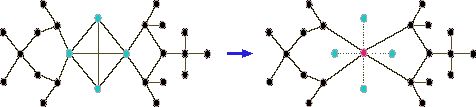
\includegraphics[height=0.9in, width=3in]{cliques.pdf}
\caption{Clique decomposition}
\label{fig:02}
\end{figure}

In our work a network is transformed by applying first the iterative k-core decomposition and then the clique decomposition.

\subsubsection*{Disjuctive interconnection graph integration} 
Given a set of graphs $\mathcal{G} = \lbrace g_1, g_,\ldots, g_n \rbrace$, we call each graph as a layer. Consider a layer tuple $g_i$, $g_j$ ($g_i, g_j \in \mathcal{G}$) and two nodes $u\in g_i,\ v \in g_j$ such that $u$ and $v$ are both represent for a same gene, we connect $u$ and $v$ by a disjuctive link. As the consequence, nodes represeting same genes in all graph layers are linked by disjuctive links. Figure \ref{fig:graph_interconnection} is a visualization for our graph integration idea.

\begin{figure}
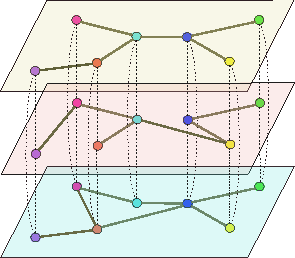
\includegraphics[height= 3in, width=3in]{multilayers.pdf}
\caption{Graph Disjunctive Interconnection Illustration}
\label{fig:03}
\end{figure}

\subsubsection{The Conjunctive Disjunctive Node Kernel}
We extend NSPDK and define a node kernel $K(G_u,G_{u'})$ between two copies of the same network $G$ where we distinguish the nodes $u$ and $u'$ respectively. The idea is to define the features of a node $u$ as the subset of NSPDK features that always have the node $u$ as one of the roots. In addition we distinguish between two types of edges, called {\em conjunctive} and {\em disjunctive} edges. When computing distances to induce neighborhood subgraphs, only conjunctive edges are considered. When choosing the
pair of neighborhoods to form a single feature, we additionally consider roots $u$ and $v$ that are not at distance $d$ but such that $u$ is connected to $w$ via a disjunctive edge and such that $w$ is at distance $d$ from $v$. In this way disjunctive edges can still allow an {\em information flow} even if their
endpoints are only considered in a pairwise fashion and not jointly. 

\begin{figure}
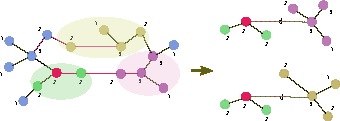
\includegraphics[height= 1.3in, width=3in]{cdnk.pdf}
\caption{CDNK}
\label{fig:04}
\end{figure}

Formally, we define two relations: the \textit{conjunctive relation} $R^{\wedge}_{r,d}(A_u, B_v, G_u)$ identical to the NSPDK relation $R_{r,d}(A_u, B_v, G)$,  and (ii) $\mathcal{D}(u,v)= d$; the \textit{disjunctive relation} $R_{r,d}^{\vee}(A_u, B_v, G_u)$ is true {\em iff} (i)  $A_u \cong \mathcal{N}_r^u$ and $B_v \cong \mathcal{N}_r^u$ are true, (ii) $\exists w$ s.t. $\mathcal{D}(w,v)= d$, and (iii) $(u,w)$ is a disjunctive edge. We define $\kappa_{r,d}$ on the  inverse relations ${R^{\wedge}_{r,d}}^{ -1}$ and ${R^{\vee}_{r,d}}^{ -1}$
\begin{center}
 $\kappa_{r,d}(G_u,G_{u'}) = \!\!\!\!\!\!\!\!\!\!\!\!
 \sum\limits_{\substack {A_u,{B}_{v} \in {R_{r,d}^{\wedge}}^{ -1}(G_u) \\ A'_{u'},{B'}_{v'} \in {R_{r,d}^{\wedge}}^{ -1}(G_{u'}) }} \!\!\!\!\!\!\!\!\!\!\!\!
  { \textbf{1}_{A_u \cong A'_{u'}} \cdot { \textbf{1}_{B_{v} \cong B'_{v'}}}}
+ \!\!\!\!\!\!\!\!\!\!\!\!
 \sum\limits_{\substack {A_u,{B}_{v} \in {R_{r,d}^{\vee}}^{ -1}(G_u) \\
  A'_{u'},{B'}_{v'} \in \ {R_{r,d}^{\vee}}^{ -1}(G_{u'}) }} \!\!\!\!\!\!\!\!\!\!\!\!
  { \textbf{1}_{A_u \cong A'_{u'}} \cdot { \textbf{1}_{B_{v} \cong B'_{v'}}}}
  $.
\end{center}
The CDNK is finally defined as $K(G_u,G_v) = \sum\limits_{r}{\sum\limits_{d}{\kappa_{r,d}(G_u,G_v)}}$, where once again for efficiency reasons, the values of $r$ and $d$ are upper bounded to a given maximal $r^*$ and $d^*$.

\subsection{Conjuctive disjuctive graph node kernel}
Here we briefly describe an efficient graph kernel called the Neighborhood Subgraph Pairs Distance kernel (NSPDK) introduced in \cite{nspdk}. NSPDK is an instance of ``decompositional'' kernels \cite{convolution-kernel} based on the idea of counting the number of common small subgraphs between two graphs. The subgraphs are pairs of neighborhoods whose roots are at a short distance. 

Given a labeled graph $G \in \mathcal{G}$ and two rooted graphs $A_u, B_v$, we first define the relation $R_{r,d}(A_u, B_v, G)$ to be true {\em iff} $A_u \cong \mathcal{N}_r^u$ is (up to isomorphism $\cong$) a neighborhood subgraph with radius $r$ of $G$ and so is $B_v \cong  \mathcal{N}_r^v$, such that $v$ is at distance $d$ from $u$: $\mathcal{D}(u,v)= d$. We then define the inverse relation $R^{-1}$ that returns all pairs of neighborhoods of radius $r$ at distance $d$ in $G$, $R^{-1}_{r,d}(G) = \lbrace A_u, B_v | R_{r,d}(A_u,B_v,G)=true\rbrace$. The kernel $\kappa_{r,d}$ over $\mathcal{G} \times \mathcal{G}$ is the number of such fragments in common in two input graphs:
\begin{center}
$\kappa_{r,d}(G,G^{'}) = 
\!\!\!\!\!\!\!\!\!\!\!\! 
\sum\limits_{\substack{A_u, B_v \ \in \ R_{r,d}^{-1}(G) \\ 
{A'}_{u'}, {B'}_{v'} \ \in \ R_{r,d}^{-1}(G')
}} \!\!\!\!\!\!\!\!\!\!\!\!  { { \textbf{1}_{A_{u} \cong A'_{u'}}} \cdot {
\textbf{1}_{B_{v} \cong B'_{v'}}} }$, 
\end{center}
\noindent where $\textbf{1}_{A \cong B}$ is the \textit{exact matching function} that returns 1 if $A$ is isomorphic to $B$ and 0 otherwise. Finally, the NSPDK is defined as $K(G,G') = \sum\limits_{r}{\sum\limits_{d}{\kappa_{r,d}(G,G')}}$, where for efficiency reasons, the values of $r$ and $d$ are upper bounded to a given maximal $r^*$ and $d^*$, respectively.

\section{Experiments}
In order to evaluate the performance of our proposed method, we conduct two separate experiments. 

The first experiment is carried out following the experimental setting in MRF. The aim of this experiment is to compare the performance of the proposed method with other existing methods for disease gene prioritization. We employ three datasets: BioGPS, Pathways and HPRD. To perform the experiments, we employed known gene-disease associations from OMIM, grouped into 20 classes on the basis of disease relatedness by Goh \emph{et al} \cite{goh}. Among those classes we selected the 12 with at least 30 confirmed genes. We then built a training set consisting of a positive set \textit{P} and a reliably negative set \textit{N} (still unlabelled in practice) for each of them. \textit{P} contains all its disease gene members. \textit{N} is constructed by randomly picking genes from known disease genes such that $\vert N \vert = \frac{1}{2} \vert P \vert$. The unknown genes relate to at least one disease class, but do not relate to the current class. We chose the genes in $N$ from the other disease genes because we assume that they were less likely to be associated to the considered class. In fact, disease genes are generally more studied and a potential association has more chances to have already been identified.

After that, leave-one-out cross validation was used to evaluate the performance of the algorithm. Iteratively, every gene in the training set was selected to be the test gene and the remaining genes in $P$ and $N$ were used to train the model. Once the model was trained, a score list for the test gene and the candidate genes was computed. Then, we computed a decision score for each test gene representing the percentage of candidate genes ranked lower than it. We collected all decision scores for every gene in all disease classes to form a global decision score list. The performance of Scuba was measured by calculating the area under the curve (AUC) in the receiver-operating-characteristic plot obtained from the decision score list. The AUC expresses the probability that a randomly chosen disease gene is ranked above a randomly picked non-disease gene for any disease class.

The second experiment (unbiased evaluation), we follow the setting used in \textit{Unbiased evaluation} with the aim at comparing our method with different web tools for disease gene prioritization. Although the first evaluation is useful to compare our method with others, predictive performance in cross-validation experiments may be inflated compared to real applications. Indeed, the retrieval of known disease genes can be facilitated by various means. One mean is the crosstalk between data repositories: for example, KEGG \cite{kegg} draws its information also from medical literature. Moreover, often the discovery of the link between a gene and a disease coincides with the discovery of a functional annotation or of a molecular interaction. In practice, instead, researchers are interested in novel associations, which in most cases are harder to find due to a lack of information around them.

In order to achieve a thorough evaluation of Scuba, we tested it in a more realistic setting, following the work of \cite{bornigen}. In this study, several gene prioritization tools were benchmarked as follows. Newly discovered disease-gene associations were collected over a timespan of six months, gathering 42 associations. As soon as a new association was discovered, eight pre-selected gene prioritization web tools were queried with a proper training set in order to mimic the discovery through each of them. These 42 predictions were used to assess the ability of the tools to successfully prioritize disease genes. The idea behind this procedure is to anticipate the integration of the associations in the data sources and so avoid biased predictions.

In order to test Scuba in this setting, we backdated our data to a time prior to May 15, 2010 by employing String v8.2 data \cite{string}. The candidate sets were constructed by considering all genes with Ensembl \cite{ensembl} gene identifier within the chromosomal regions around the test genes, in order to get on average 100 candidates for each trial. Then, we performed prioritizations for each test gene in two distinct cases - genome-wide and candidate set-based prioritizations. In genome-wide prioritizations all coding genes in the genome were prioritized, while in candidate set-based tests only the genes belonging to the candidate groups were ranked. In both cases, we normalized ranking positions over the total number of genes in order to get the median and the standard deviation of the normalized ranks for test genes. We also computed the true positive rate (TPR) relatively to some representative thresholds (5\%, 10\% and 30\% of the ranking) and the AUC obtained by averaging over the 42 prioritizations.

\subsection*{Data sources}
\begin{itemize}
	\item \textbf{Human Protein Reference Database} (\textbf{HPRD}): The HPRD resource provides protein interaction data which we implement as an unweighted graph, where genes are linked if their corresponding proteins interact.
	\item \textbf{BioGPS}: It contains expression profiles for 79 human tissues, which are measured by using the Affymetrix U133A array. Gene co-expression, defined by pairwise Pearson correlation coefficients (PCC), is used to build an unweighted graph. A pair of genes are linked by an edge if the PCC value is larger than 0.5.
	\item \textbf{Pathways}: Pathway datasets are obtained from the database of KEGG, Reactome, PharmGKB and PID, which contain 280, 1469, 99 and 2679 pathways, respectively. A pathway co-participation network is constructed by connecting genes that co-participate in any pathway.
	\item \textbf{String}: The String database gathers protein information covering seven levels of evidence: genomic proximity in procaryotes, fused genes, co-occurrence in organisms, co-expression, experimentally validated physical interactions, external databases and text mining. Overall, these aspects focus on functional relationships that can be seen as edges of a weighted graph, where the weight is given by the reliability of that relationship. To perform the unbiased evaluation we employed the version 8.2 of String, from which we extracted functional links among 17078 human genes.
	\item \textbf{Omim}: OMIM is a public database of disease-gene association. Genes
implicated in the same disease are more likely to be involved in other
similar diseases as well. Therefore, Omim network is formed by connecting genes which are involved in common disease(s).
\end{itemize}
\section{Results and Discussion}
Table \ref{tab:1} and \ref{tab:2} show the performance of our proposed method together with different methods and tools in two experimental settings. It can be seen from tables that DIGI outperforms all compared methods in all cases. In the first experiment, it shows a bit higher than the second best one, Scuba and much higher than the rest of methods. In particular, DIGI shows around 5$\%$ higher than MRF and more than 15$\%$ compared to DIR and GeneWanderer. In the table \ref{tab:2}, it presents impressive results in both Genome wide and Candidate-based settings. In disease gene prioritization, we pay more attention to the top genes in the ranking since we normally consider them to have actual medical tests to determin the relation of genes with a given genetic disease due to the time and financial constraints. The performance of DIGI on top 5$\%$ and 10$\%$ is far more higher than all tools and methods. Its average medians are only 6.56 and 8.00 for Genome wide and Candidate genes settings, respectively. In Genome wide setting, DIGI's average AUC performance is about 6$\%$ higher than the second best one, Scuba, meanwhile in candidate genes setting, it together with GeneDistiller are ranked first with 0.85.
\begin{table*}
  \caption{Performance of different methods on MRF experimental setting}
  \label{tab:1}
  \begin{tabular}{cccccl}
    \toprule
    Method & \textbf{DIGI} & DIR & F3PC & MRF & Scuba \\
    \midrule
    AUC & \textbf{0.881} & 0.716 & 0.830 & 0.731 & 0.876 \\    
    \bottomrule
  \end{tabular}
\end{table*}


\begin{table*}
\caption{Performance of DIGI comparing with Scuba and other web tools on unbiased setting} 
\label{tab:2}
%\setlength\tabcolsep{0pt} % let LaTeX compute intercolumn whitespace
%
%\centering
%\smallskip 
\begin{tabular*}{\textwidth}{@{\extracolsep{\fill}}ccccccl}
\hline
  Tool/Method & Response & Rank & TPR in top & TPR in top & TPR in top & AUC\\
              & rate     & median & 5\% (\%) & 10\% (\%) & 30\% (\%) &\\
\hline
Genome-Wide \\
  \textbf{DIGI} & 100 & \textbf{6.56} & \textbf{42.8} & \textbf{63.3} & \textbf{83.3} & \textbf{86.1} \\
  Scuba & 100 & 10.55  &  33.3 & 47.6 & 78.6 & 0.80 \\
  Candid & 100 &  18.10 & 21.4 & 33.3 & 64.3 & 0.73 \\
  Endeavour & 100 &  15.49 & 28.6 & 38.1 & 71.4 & 0.79 \\  
  Pinta & 100 & 19.03 & 26.2 & 31.0 & 71.4 & 0.77 \\
  \hline
  Candidate-Genes \\
  DIGI & 100 &  \textbf{8.00} & \textbf{38.1} & \textbf{59.5} & 83.3 & \textbf{0.85} \\
  Scuba & 100 &  12.95  &  28.6 & 45.2 & 73.8 & 0.78 \\
  Suspects & 88.9$^a$ &  12.77$^a$ & 33.3$^a$ & 33.3$^a$ & 63.0$^a$ & 0.76$^a$ \\
  ToppGene & 97.6 &  16.80 & 35.7 & 42.9 & 52.4 & 0.66 \\  
  GeneWanderer-RW & 88.1 &  22.10 & 16.7 & 26.2 & 61.9 & 0.71 \\
  Posmed-KS & 47.6 &  31.44 & 4.7 & 7.1 & 23.8 & 0.58 \\
  GeneDistiller & 97.6 &  11.11 & 26.2 & 47.6 & 78.6 & \textbf{0.85}\\  
  Endeavour & 100 &  11.16 & 26.2 & 42.9 & \textbf{90.5} & 0.82 \\
  Pinta & 100 & 18.87 & 28.6 & 31.0 & 71.4 & 0.75 \\  
\hline
\end{tabular*}
\end{table*}

\section{Conclusion}
We have proposed an efficient method for disease gene prioritization.

\begin{acks}
This work was supported by the University of Padova, Strategic Project BIOINFOGEN

\end{acks}

%\section{The Body of The Paper}
%Typically, the body of a paper is organized into a hierarchical
%structure, with numbered or unnumbered headings for sections,
%subsections, sub-subsections, and even smaller sections.  The command
%\texttt{{\char'134}section} that precedes this paragraph is part of
%such a hierarchy.\footnote{This is a footnote.} \LaTeX\ handles the
%numbering and placement of these headings for you, when you use the
%appropriate heading commands around the titles of the headings.  If
%you want a sub-subsection or smaller part to be unnumbered in your
%output, simply append an asterisk to the command name.  Examples of
%both numbered and unnumbered headings will appear throughout the
%balance of this sample document.
%
%Because the entire article is contained in the \textbf{document}
%environment, you can indicate the start of a new paragraph with a
%blank line in your input file; that is why this sentence forms a
%separate paragraph.
%
%\subsection{Type Changes and {\itshape Special} Characters}
%
%We have already seen several typeface changes in this sample.  You can
%indicate italicized words or phrases in your text with the command
%\texttt{{\char'134}textit}; emboldening with the command
%\texttt{{\char'134}textbf} and typewriter-style (for instance, for
%computer code) with \texttt{{\char'134}texttt}.  But remember, you do
%not have to indicate typestyle changes when such changes are part of
%the \textit{structural} elements of your article; for instance, the
%heading of this subsection will be in a sans serif\footnote{Another
%  footnote here.  Let's make this a rather long one to see how it
%  looks.} typeface, but that is handled by the document class file.
%Take care with the use of\footnote{Another footnote.}  the
%curly braces in typeface changes; they mark the beginning and end of
%the text that is to be in the different typeface.
%
%You can use whatever symbols, accented characters, or non-English
%characters you need anywhere in your document; you can find a complete
%list of what is available in the \textit{\LaTeX\ User's Guide}
%\cite{Lamport:LaTeX}.
%
%\subsection{Math Equations}
%You may want to display math equations in three distinct styles:
%inline, numbered or non-numbered display.  Each of
%the three are discussed in the next sections.
%
%\subsubsection{Inline (In-text) Equations}
%A formula that appears in the running text is called an
%inline or in-text formula.  It is produced by the
%\textbf{math} environment, which can be
%invoked with the usual \texttt{{\char'134}begin\,\ldots{\char'134}end}
%construction or with the short form \texttt{\$\,\ldots\$}. You
%can use any of the symbols and structures,
%from $\alpha$ to $\omega$, available in
%\LaTeX~\cite{Lamport:LaTeX}; this section will simply show a
%few examples of in-text equations in context. Notice how
%this equation:
%\begin{math}
%  \lim_{n\rightarrow \infty}x=0
%\end{math},
%set here in in-line math style, looks slightly different when
%set in display style.  (See next section).
%
%\subsubsection{Display Equations}
%A numbered display equation---one set off by vertical space from the
%text and centered horizontally---is produced by the \textbf{equation}
%environment. An unnumbered display equation is produced by the
%\textbf{displaymath} environment.
%
%Again, in either environment, you can use any of the symbols
%and structures available in \LaTeX\@; this section will just
%give a couple of examples of display equations in context.
%First, consider the equation, shown as an inline equation above:
%\begin{equation}
%  \lim_{n\rightarrow \infty}x=0
%\end{equation}
%Notice how it is formatted somewhat differently in
%the \textbf{displaymath}
%environment.  Now, we'll enter an unnumbered equation:
%\begin{displaymath}
%  \sum_{i=0}^{\infty} x + 1
%\end{displaymath}
%and follow it with another numbered equation:
%\begin{equation}
%  \sum_{i=0}^{\infty}x_i=\int_{0}^{\pi+2} f
%\end{equation}
%just to demonstrate \LaTeX's able handling of numbering.
%
%\subsection{Citations}
%Citations to articles~\cite{bowman:reasoning,
%clark:pct, braams:babel, herlihy:methodology},
%conference proceedings~\cite{clark:pct} or maybe
%books \cite{Lamport:LaTeX, salas:calculus} listed
%in the Bibliography section of your
%article will occur throughout the text of your article.
%You should use BibTeX to automatically produce this bibliography;
%you simply need to insert one of several citation commands with
%a key of the item cited in the proper location in
%the \texttt{.tex} file~\cite{Lamport:LaTeX}.
%The key is a short reference you invent to uniquely
%identify each work; in this sample document, the key is
%the first author's surname and a
%word from the title.  This identifying key is included
%with each item in the \texttt{.bib} file for your article.
%
%The details of the construction of the \texttt{.bib} file
%are beyond the scope of this sample document, but more
%information can be found in the \textit{Author's Guide},
%and exhaustive details in the \textit{\LaTeX\ User's
%Guide} by Lamport~\shortcite{Lamport:LaTeX}.
%
%This article shows only the plainest form
%of the citation command, using \texttt{{\char'134}cite}.
%
%Some examples.  A paginated journal article \cite{Abril07}, an enumerated
%journal article \cite{Cohen07}, a reference to an entire issue \cite{JCohen96},
%a monograph (whole book) \cite{Kosiur01}, a monograph/whole book in a series (see 2a in spec. document)
%\cite{Harel79}, a divisible-book such as an anthology or compilation \cite{Editor00}
%followed by the same example, however we only output the series if the volume number is given
%\cite{Editor00a} (so Editor00a's series should NOT be present since it has no vol. no.),
%a chapter in a divisible book \cite{Spector90}, a chapter in a divisible book
%in a series \cite{Douglass98}, a multi-volume work as book \cite{Knuth97},
%an article in a proceedings (of a conference, symposium, workshop for example)
%(paginated proceedings article) \cite{Andler79}, a proceedings article
%with all possible elements \cite{Smith10}, an example of an enumerated
%proceedings article \cite{VanGundy07},
%an informally published work \cite{Harel78}, a doctoral dissertation \cite{Clarkson85},
%a master's thesis: \cite{anisi03}, an online document / world wide web
%resource \cite{Thornburg01, Ablamowicz07, Poker06}, a video game (Case 1) \cite{Obama08} and (Case 2) \cite{Novak03}
%and \cite{Lee05} and (Case 3) a patent \cite{JoeScientist001},
%work accepted for publication \cite{rous08}, 'YYYYb'-test for prolific author
%\cite{SaeediMEJ10} and \cite{SaeediJETC10}. Other cites might contain
%'duplicate' DOI and URLs (some SIAM articles) \cite{Kirschmer:2010:AEI:1958016.1958018}.
%Boris / Barbara Beeton: multi-volume works as books
%\cite{MR781536} and \cite{MR781537}.
%
%A couple of citations with DOIs: \cite{2004:ITE:1009386.1010128,
%  Kirschmer:2010:AEI:1958016.1958018}. 
%
%Online citations: \cite{TUGInstmem, Thornburg01, CTANacmart}.  
%
%
%\subsection{Tables}
%Because tables cannot be split across pages, the best
%placement for them is typically the top of the page
%nearest their initial cite.  To
%ensure this proper ``floating'' placement of tables, use the
%environment \textbf{table} to enclose the table's contents and
%the table caption.  The contents of the table itself must go
%in the \textbf{tabular} environment, to
%be aligned properly in rows and columns, with the desired
%horizontal and vertical rules.  Again, detailed instructions
%on \textbf{tabular} material
%are found in the \textit{\LaTeX\ User's Guide}.
%
%Immediately following this sentence is the point at which
%Table~\ref{tab:freq} is included in the input file; compare the
%placement of the table here with the table in the printed
%output of this document.
%
%\begin{table}
%  \caption{Frequency of Special Characters}
%  \label{tab:freq}
%  \begin{tabular}{ccl}
%    \toprule
%    Non-English or Math&Frequency&Comments\\
%    \midrule
%    \O & 1 in 1,000& For Swedish names\\
%    $\pi$ & 1 in 5& Common in math\\
%    \$ & 4 in 5 & Used in business\\
%    $\Psi^2_1$ & 1 in 40,000& Unexplained usage\\
%  \bottomrule
%\end{tabular}
%\end{table}
%
%To set a wider table, which takes up the whole width of the page's
%live area, use the environment \textbf{table*} to enclose the table's
%contents and the table caption.  As with a single-column table, this
%wide table will ``float'' to a location deemed more desirable.
%Immediately following this sentence is the point at which
%Table~\ref{tab:commands} is included in the input file; again, it is
%instructive to compare the placement of the table here with the table
%in the printed output of this document.
%
%
%\begin{table*}
%  \caption{Some Typical Commands}
%  \label{tab:commands}
%  \begin{tabular}{ccl}
%    \toprule
%    Command &A Number & Comments\\
%    \midrule
%    \texttt{{\char'134}author} & 100& Author \\
%    \texttt{{\char'134}table}& 300 & For tables\\
%    \texttt{{\char'134}table*}& 400& For wider tables\\
%    \bottomrule
%  \end{tabular}
%\end{table*}
%% end the environment with {table*}, NOTE not {table}!
%
%It is strongly recommended to use the package booktabs~\cite{Fear05}
%and follow its main principles of typography with respect to tables:
%\begin{enumerate}
%\item Never, ever use vertical rules.
%\item Never use double rules.
%\end{enumerate}
%It is also a good idea not to overuse horizontal rules.
%
%
%\subsection{Figures}
%
%Like tables, figures cannot be split across pages; the best placement
%for them is typically the top or the bottom of the page nearest their
%initial cite.  To ensure this proper ``floating'' placement of
%figures, use the environment \textbf{figure} to enclose the figure and
%its caption.
%
%This sample document contains examples of \texttt{.eps} files to be
%displayable with \LaTeX.  If you work with pdf\LaTeX, use files in the
%\texttt{.pdf} format.  Note that most modern \TeX\ systems will convert
%\texttt{.eps} to \texttt{.pdf} for you on the fly.  More details on
%each of these are found in the \textit{Author's Guide}.
%
%\begin{figure}
%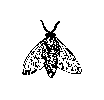
\includegraphics{fly}
%\caption{A sample black and white graphic.}
%\end{figure}
%
%\begin{figure}
%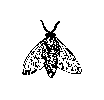
\includegraphics[height=1in, width=1in]{fly}
%\caption{A sample black and white graphic
%that has been resized with the \texttt{includegraphics} command.}
%\end{figure}
%
%
%As was the case with tables, you may want a figure that spans two
%columns.  To do this, and still to ensure proper ``floating''
%placement of tables, use the environment \textbf{figure*} to enclose
%the figure and its caption.  And don't forget to end the environment
%with \textbf{figure*}, not \textbf{figure}!
%
%\begin{figure*}
%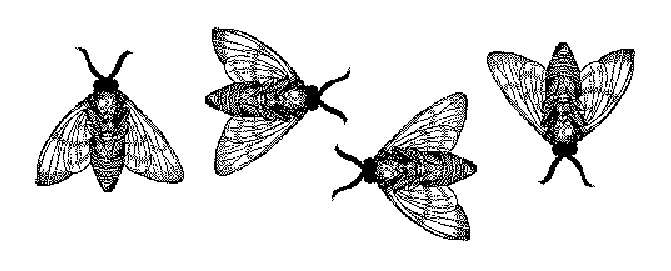
\includegraphics{flies}
%\caption{A sample black and white graphic
%that needs to span two columns of text.}
%\end{figure*}
%
%
%\begin{figure}
%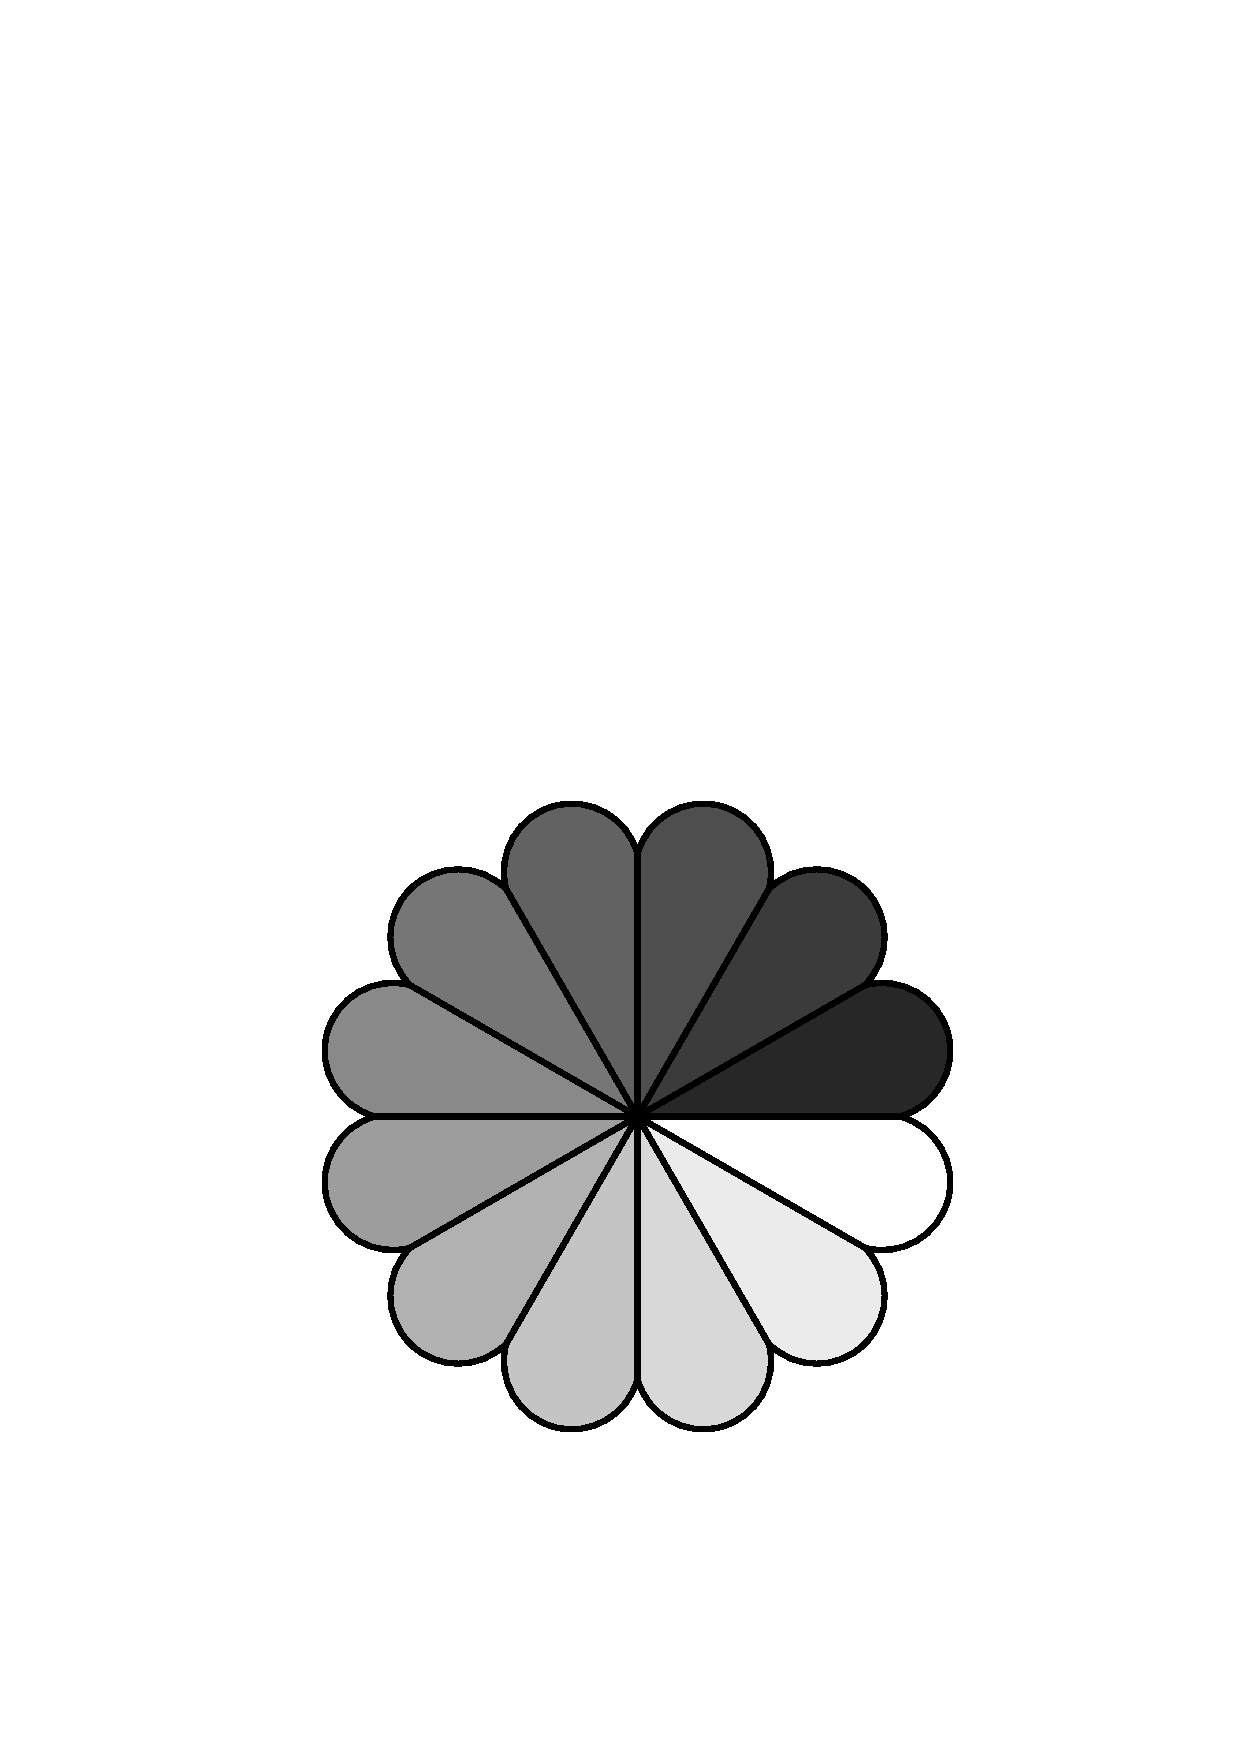
\includegraphics[height=1in, width=1in]{rosette}
%\caption{A sample black and white graphic that has
%been resized with the \texttt{includegraphics} command.}
%\end{figure}
%
%\subsection{Theorem-like Constructs}
%
%Other common constructs that may occur in your article are the forms
%for logical constructs like theorems, axioms, corollaries and proofs.
%ACM uses two types of these constructs:  theorem-like and
%definition-like.
%
%Here is a theorem:
%\begin{theorem}
%  Let $f$ be continuous on $[a,b]$.  If $G$ is
%  an antiderivative for $f$ on $[a,b]$, then
%  \begin{displaymath}
%    \int^b_af(t)\,dt = G(b) - G(a).
%  \end{displaymath}
%\end{theorem}
%
%Here is a definition:
%\begin{definition}
%  If $z$ is irrational, then by $e^z$ we mean the
%  unique number that has
%  logarithm $z$:
%  \begin{displaymath}
%    \log e^z = z.
%  \end{displaymath}
%\end{definition}
%
%The pre-defined theorem-like constructs are \textbf{theorem},
%\textbf{conjecture}, \textbf{proposition}, \textbf{lemma} and
%\textbf{corollary}.  The pre-defined de\-fi\-ni\-ti\-on-like constructs are
%\textbf{example} and \textbf{definition}.  You can add your own
%constructs using the \textsl{amsthm} interface~\cite{Amsthm15}.  The
%styles used in the \verb|\theoremstyle| command are \textbf{acmplain}
%and \textbf{acmdefinition}.
%
%Another construct is \textbf{proof}, for example,
%
%\begin{proof}
%  Suppose on the contrary there exists a real number $L$ such that
%  \begin{displaymath}
%    \lim_{x\rightarrow\infty} \frac{f(x)}{g(x)} = L.
%  \end{displaymath}
%  Then
%  \begin{displaymath}
%    l=\lim_{x\rightarrow c} f(x)
%    = \lim_{x\rightarrow c}
%    \left[ g{x} \cdot \frac{f(x)}{g(x)} \right ]
%    = \lim_{x\rightarrow c} g(x) \cdot \lim_{x\rightarrow c}
%    \frac{f(x)}{g(x)} = 0\cdot L = 0,
%  \end{displaymath}
%  which contradicts our assumption that $l\neq 0$.
%\end{proof}
%
%\section{Conclusions}
%This paragraph will end the body of this sample document.
%Remember that you might still have Acknowledgments or
%Appendices; brief samples of these
%follow.  There is still the Bibliography to deal with; and
%we will make a disclaimer about that here: with the exception
%of the reference to the \LaTeX\ book, the citations in
%this paper are to articles which have nothing to
%do with the present subject and are used as
%examples only.
%%\end{document}  % This is where a 'short' article might terminate
%
%
%
%\appendix
%%Appendix A
%\section{Headings in Appendices}
%The rules about hierarchical headings discussed above for
%the body of the article are different in the appendices.
%In the \textbf{appendix} environment, the command
%\textbf{section} is used to
%indicate the start of each Appendix, with alphabetic order
%designation (i.e., the first is A, the second B, etc.) and
%a title (if you include one).  So, if you need
%hierarchical structure
%\textit{within} an Appendix, start with \textbf{subsection} as the
%highest level. Here is an outline of the body of this
%document in Appendix-appropriate form:
%\subsection{Introduction}
%\subsection{The Body of the Paper}
%\subsubsection{Type Changes and  Special Characters}
%\subsubsection{Math Equations}
%\paragraph{Inline (In-text) Equations}
%\paragraph{Display Equations}
%\subsubsection{Citations}
%\subsubsection{Tables}
%\subsubsection{Figures}
%\subsubsection{Theorem-like Constructs}
%\subsubsection*{A Caveat for the \TeX\ Expert}
%\subsection{Conclusions}
%\subsection{References}
%Generated by bibtex from your \texttt{.bib} file.  Run latex,
%then bibtex, then latex twice (to resolve references)
%to create the \texttt{.bbl} file.  Insert that \texttt{.bbl}
%file into the \texttt{.tex} source file and comment out
%the command \texttt{{\char'134}thebibliography}.
%% This next section command marks the start of
%% Appendix B, and does not continue the present hierarchy
%\section{More Help for the Hardy}
%
%Of course, reading the source code is always useful.  The file
%\path{acmart.pdf} contains both the user guide and the commented
%code.
%
%\begin{acks}
%  The authors would like to thank Dr. Yuhua Li for providing the
%  matlab code of  the \textit{BEPS} method. 
%
%  The authors would also like to thank the anonymous referees for
%  their valuable comments and helpful suggestions. The work is
%  supported by the \grantsponsor{GS501100001809}{National Natural
%    Science Foundation of
%    China}{http://dx.doi.org/10.13039/501100001809} under Grant
%  No.:~\grantnum{GS501100001809}{61273304}
%  and~\grantnum[http://www.nnsf.cn/youngscientsts]{GS501100001809}{Young
%    Scientsts' Support Program}.
%
%\end{acks}
